\documentclass[italian,12pt,a4paper]{article}
\usepackage[utf8]{inputenc}
\usepackage[T1]{fontenc}
\usepackage{mathtools}
\usepackage{blkarray, bigstrut} %
\usepackage{babel}
\usepackage{graphicx}
\usepackage{subfig}
\usepackage{hyperref}
\usepackage{colortbl}
\usepackage{algorithm}
\usepackage{algpseudocode}
\usepackage{algorithmicx}
\usepackage{tabularx}
\usepackage[backend=bibtex,sorting=none]{biblatex}
\addbibresource{citations.bib}
\title{Università degli studi di Bari facoltà di scienze MM.FF.NN}
\date{} % clear date
\hypersetup{
	colorlinks=true,
	linkcolor=black,
	filecolor=magenta,      
	urlcolor=cyan,
	citecolor=cyan,
	pdfpagemode=FullScreen,
}
\graphicspath{ {./img/} }
\RequirePackage[subfigure]{tocloft}

\cftsetindents{section}{0em}{2em}
\cftsetindents{subsection}{0em}{2em}

\renewcommand\cfttoctitlefont{\hfill\Large\bfseries}
\renewcommand\cftaftertoctitle{\hfill\mbox{}}

\setcounter{tocdepth}{2}
\begin{document}
	\maketitle
	\thispagestyle{empty}
	\begin{center}
		\huge	\textbf{Progetto ingegneria della conoscenza}
		\linebreak
		\linebreak
		\Large \textbf{TrainDelay-project}
	\end{center}
	
	\begin{center}
		by \\
		\Large \textbf{Vito Proscia mat. 735975} \\
	\end{center}
	\vspace{4px}
	\begin{center}
		Email: \href{mailto:v.proscia3@studenti.uniba.it}{v.proscia3@studenti.uniba.it}
	\end{center}
	\vspace{50px}
	\begin{figure}[hb]
		\centering
		
\includegraphics[width=5cm]{image.png}
	\end{figure}
	\vspace{50px}
	\begin{center}
		Repository github: \href{https://github.com/Giut0/TrainDelay-project}{TrainDelay-project}
	\end{center}
	
	\vfill
	\begin{center}
		Anno accadenico 2022-2023
	\end{center}
	
	\newpage
	
	\tableofcontents

	\newpage

	\section{Introduzione}
	
	\subsection{Definizione obiettivo principale}
	
	L'obiettivo principale del progetto è la creazione di un motore di ricerca che trova i migliori itinerari di viaggio in treno sulla base della stazione di partenza e di arrivo e che, per ogni viaggio, mostra una predizione del probabile ritardo.\\
	Questo sistema non solo potrà far risparmiare del tempo a chi organizza dei viaggi valutando ogni singola tratta, ma garantirà un risparmio econimico ai viaggiatori garantendo che la tratta scelta dal sistema sia la minima e necessaria per arrivare alla destinazione, inoltre la predizione del ritardo andrà a ridurre in maniera significativa il disagio da parte dei viaggiatori. 
	
	
	\subsection{Tool utilizzati}
	Per la sperimentazione sono stati usati diversi stumenti/librerie, i principali sono:
	
		\begin{itemize}
			\item \textbf{PySWIP}, libreria Python che fornisce un'interfaccia per utilizzare SWI-Prolog, usato per la rappreesentazione formale della schedul dei treni;
			\item \textbf{NetworkX}, libreria Python utilizzata per la creazione, l'analisi e la manipolazione di reti complesse. Questa libreria fornisce un insieme di strumenti per la rappresentazione di reti e grafi, oltre a un'ampia gamma di algoritmi e funzioni per eseguire diverse operazioni su di essi;
			\item \textbf{Scikit-learn}, libreria open-source che fornisce un vasto insieme di strumenti nell'ambito del machine learning e dell'apprendimento automatico.
		\end{itemize}

	\section{Rappresentazione formale della conoscenza}
	
	La rappresentazione formale della conoscenza è importante per consentire l'espressione della conoscenza in modo preciso, organizzato e interpretabile da parte di sistemi informatici.\\
	Per gestire formalmente la conoscenza, facilitando la ricerca e l'accesso a informazioni specifiche, si costruisce una \textbf{knowledge base} (base di conoscenza), una raccolta strutturata di informazioni o dati che rappresenta la conoscenza su un determinato dominio o argomento, utilizzate per immagazzinare e organizzare la conoscenza in modo che sia accessibile e utilizzabile da sistemi informatici.
	
	\subsection{Origine dei dati}
	Tutte le informazioni relative allo schedul dei treni sono state reperite per mezzo dell'interrogazione alle API messe a disposizione dal sito \href{http://www.viaggiatreno.it/infomobilita/index.jsp}{www.viaggiatreno.it}, mentre le informazioni relative alle stazioni sono state recuperate dal repository "trenitalia: scraping di viaggiatreno".\cite{dati_stazioni}
	
	\subsection{Descrizione dei dati}
	La parte iniziale del progetto si è concentarta sulla rappresentazione formale attraverso fatti e regole Prolog (linguaggio di programmazione logica utilizzato per definire relazioni tra fatti e regole attraverso la logica dei predicati) dello schedule dei treni e delle stazioni, in particolare ogni treno si è ritenuto opportuno caratterizzarlo da:
	
		\begin{enumerate}
			\item \textit{ID treno} identificatore univoco del treno;
			\item \textit{Tipo di treno} regionale o nazionale;
			\item \textit{ID stazione di partenza};
			\item \textit{ID stazione di arrivo};
			\item\textit{Orario di partenza} (HH:MM);
			\item \textit{Orario di arrivo} (HH:MM);
			\item \textit{Lista delle fermate}.
		\end{enumerate} 
		\vspace{20px}
		Di seguito è riportato un esempio:
		
		\begin{figure}[!h]
			\centering
			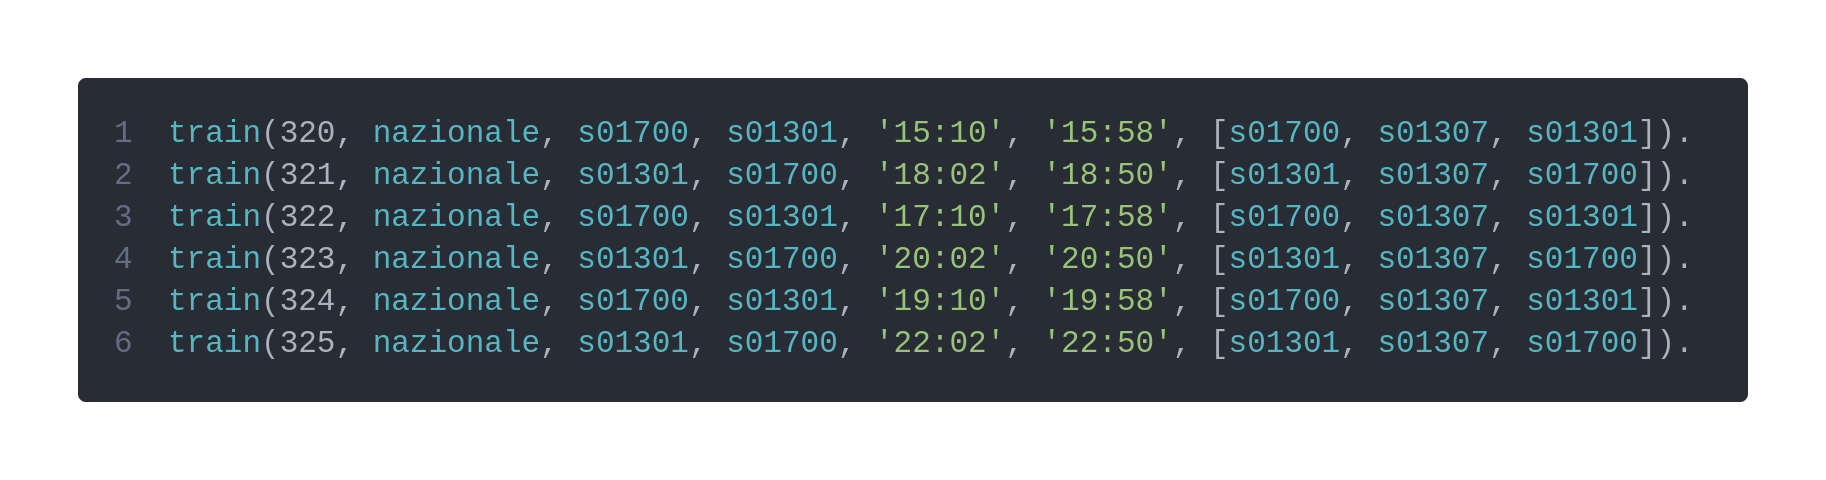
\includegraphics[width=400px]{img/code_prolog1}
			\caption{Esempio di rappresentazione formale dello shedule dei treni}
		\end{figure}
		\newpage
	Mentre ogni stazione si è pensato caratterizzarla da:
	
		\begin{enumerate}
			\item \textit{ID stazione}, identificatore univoco delle stazioni;
			\item \textit{Nome stazione};
			\item \textit{Regione stazione}.
		\end{enumerate}
		Di seguito è riportato un esempio:
	
		\begin{figure}[!h]
			\centering
			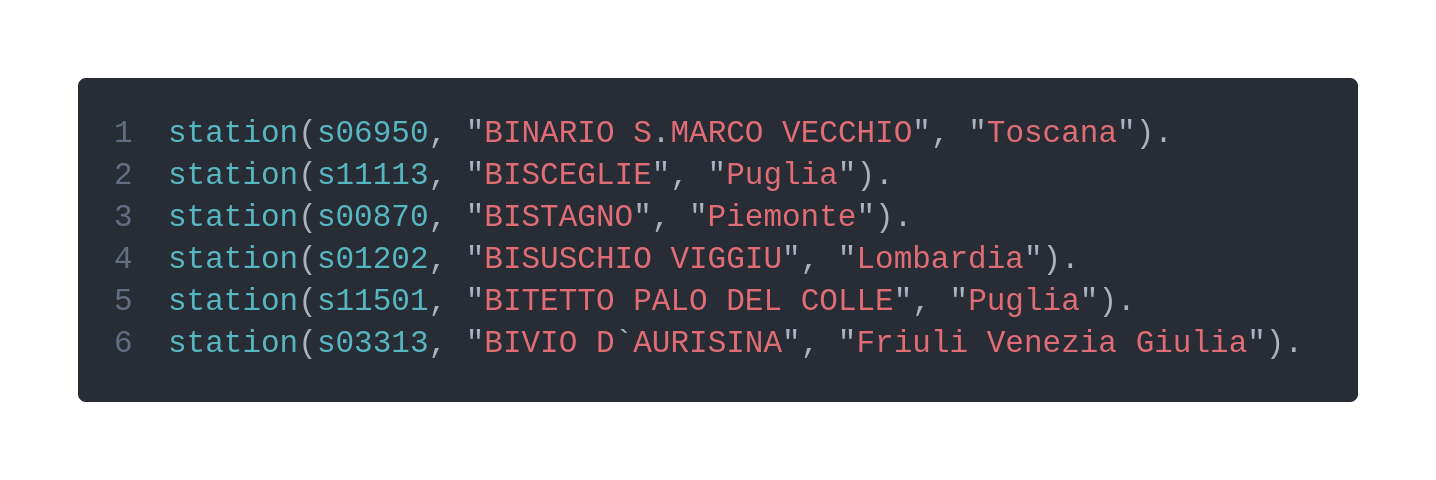
\includegraphics[width=400px]{img/code_prolog2}
			\caption{Esempio di rappresentazione formale delle stazioni}
		\end{figure}
		\vspace{10px}
		\setlength{\parindent}{0cm}
		Questa rappresentazione dei treni e delle stazioni nel linguaggio di programmazione logica ha fornito una base solida per la gestione e l'analisi dei dati ferroviari. \\
		\linebreak
		Con questa struttura dati, è stato possibile effettuare interrogazioni, trovare treni tra stazioni, e condurre altre operazioni analitiche necessarie per il progetto.

\subsection{Rappresentazione basata su grafo}

\subsubsection{Costruzione grafo}
	Per la possibilità di ricercare l'itinerario di viaggio migliore, cioè con il numero minimo di stazioni, si è pensato di costruire un grafo delle stazioni, dove ogni nodo rappresenta una stazione diversa (\texttt{idStazione}) e la presenza di un arco tra due nodi si traduce in un collegamento ferroviario tra le due stazioni.
	\\
	\begin{figure}[t]
		\centering
		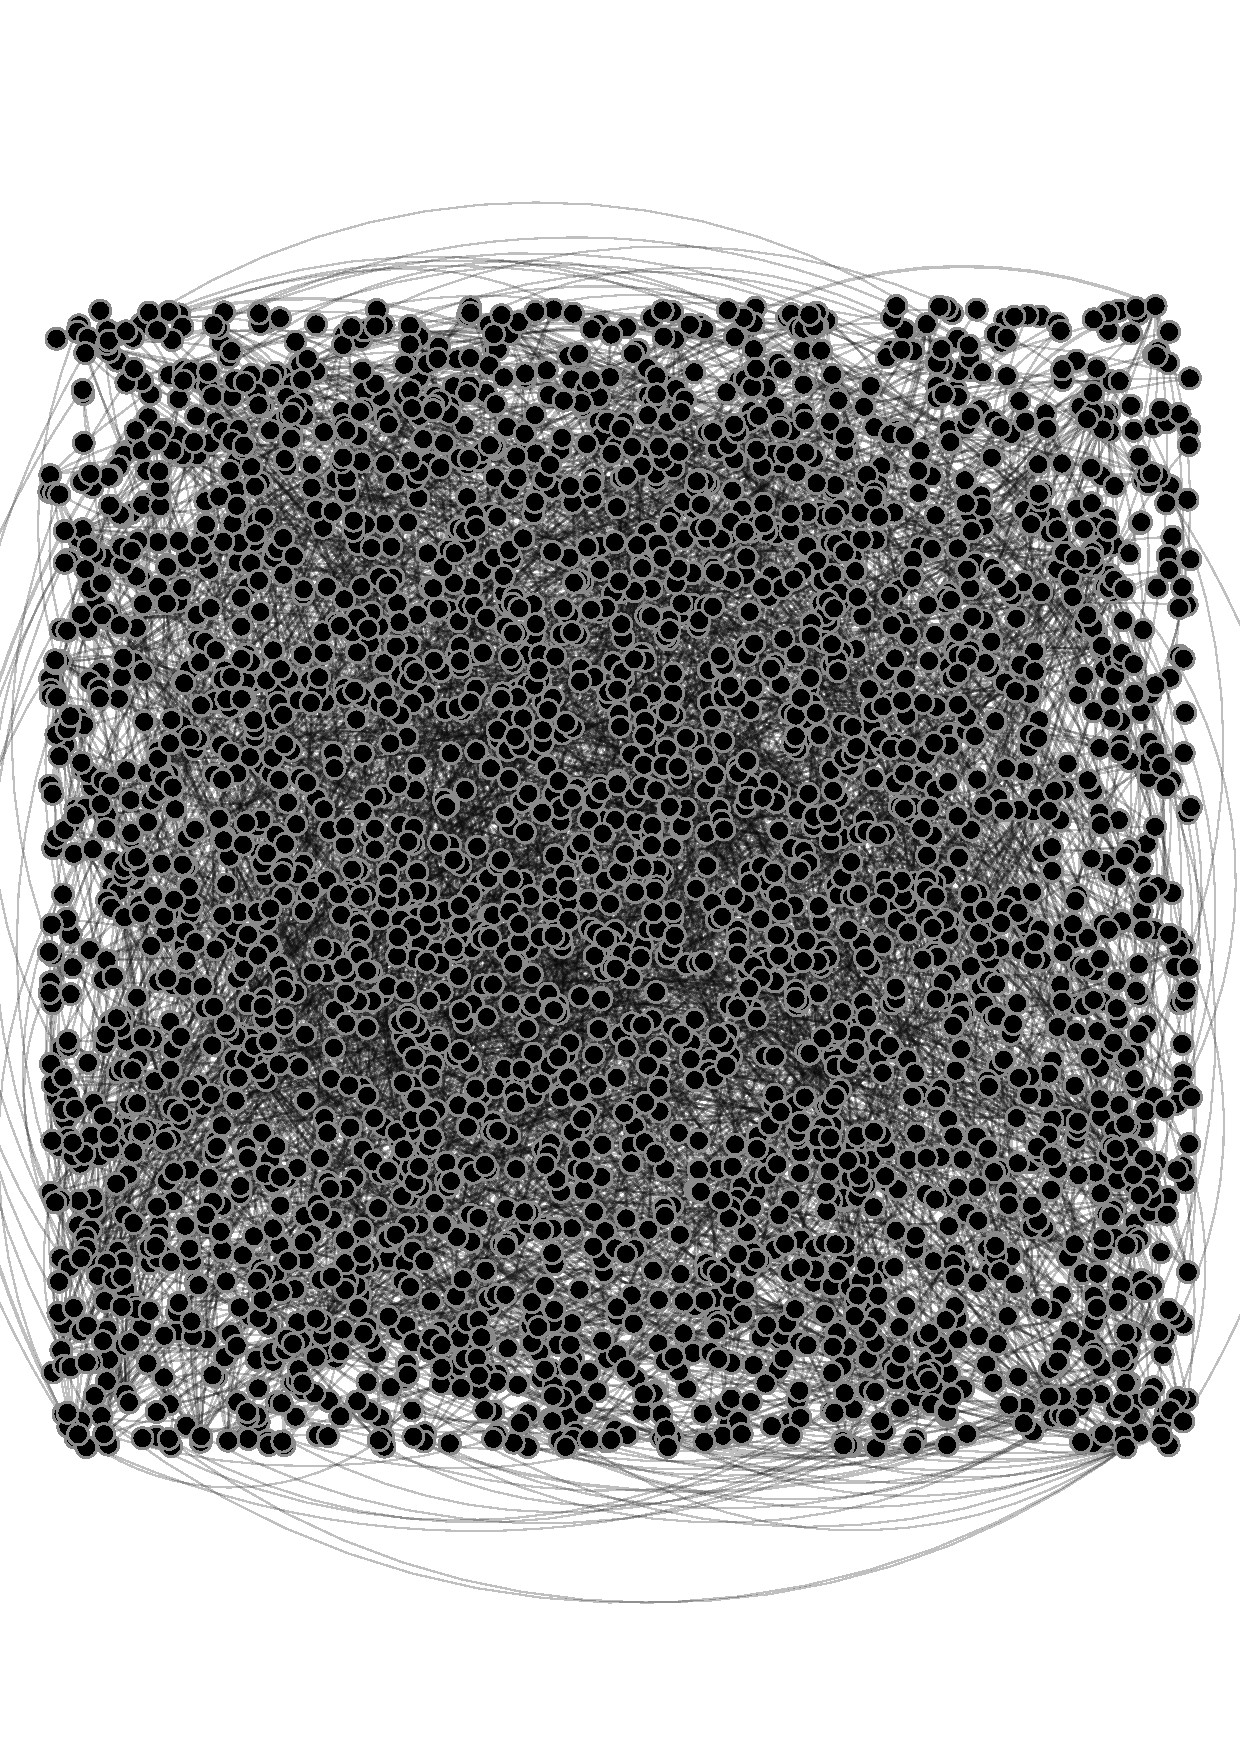
\includegraphics[width=220px]{img/stations}
		\caption{Grafo delle stazioni}
		\label{fig:stationsgraph}
	\end{figure}
	
\subsubsection{Ricerca grafo}
	
		Per la ricerca del percorso più breve tra due stazioni si è utilizzato \textbf{l'algoritmo di Dijkstra}, un algoritmo di ricerca del cammino più breve in un grafo pesato con pesi non negativi, in questo caso specifico il peso di ogni arco è 1, quindi l'algortmo cercherà il percorso con il più breve numero di nodi.\\
		Inizia da un nodo sorgente e calcola le distanze minime da esso a tutti gli altri nodi, mantenendo una coda di priorità, durante l'esecuzione, visita i nodi adiacenti al nodo corrente e aggiorna le distanze minime se trova un cammino più breve. Implementato dalla libreria \textbf{NetworkX} che restituisce il percorso più breve sotto forma di lista di nodi. \\
		\linebreak
		Anche se il grao prodotto non è propriamente pesato, si è pensato di usare l'algoritmo di Dijkstra, per una possibile estensione e miglioramento del sistema convertendo il grafo attuale in uno pesato, magari andando ad impostare come pesi degli archi le distanze che intercorrono tra le stazioni collegate.
		
	\begin{algorithm}[h]
		\caption{Algoritmo di Dijkstra}
		\begin{algorithmic}[1]
			\Procedure{Dijkstra}{$G, s$}
			\State $dist \gets$ array di distanze inizializzato a $\infty$ per tutti i nodi
			\State $dist[s] \gets 0$
			\State $S \gets$ insieme vuoto dei nodi visitati
			\While{$S$ non contiene tutti i nodi}
			\State $u \gets$ nodo non visitato con la minima distanza in $dist$
			\State Aggiungi $u$ a $S$
			\ForAll{nodi adiacenti $v$ di $u$}
			\State $alt \gets dist[u] +$ peso dell'arco tra $u$ e $v$
			\If{$alt < dist[v]$}
			\State $dist[v] \gets alt$
			\EndIf
			\EndFor
			\EndWhile
			\State \textbf{return} $dist$ 
			\EndProcedure
		\end{algorithmic}
	\end{algorithm}
	\vspace{200px}
	
	\begin{table}[h]
		\centering
		\begin{tabular}{|l|l|}
			\hline
			\textbf{Operazione} & \textbf{Complessità} \\ \hline
			Inizializzazione & $O(V)$ \\ \hline
			Inserimento di nodi nella coda & $O(V \log V)$ \\ \hline
			Estrazione del nodo con distanza minima & $O(\log V)$ \\ \hline
			Aggiornamento delle distanze & $O(E \log V)$ \\ \hline
			Totale & $O((V + E) \log V)$ \\ \hline
		\end{tabular}
		\caption{Complessità dell'algoritmo di Dijkstra con heap binario}
	\end{table}
	
	\vspace{20px}

	\subsection{Query Knowledge base}
	Per andare ad interagire un Knowledge base vengono eseguite delle \textbf{query}, interrogazioni alla KB, che permettono di estrapolare informazioni specifiche.\\
	In questo caso sono state messe a disposizione delle query predefinite per poter recuperare le informazioni relative ai treni secondo le esigenze dell'utente. \\
	In particolare sono state pensate quattro query principali, che che verranno eseguite in base alle esigenze dell'utente correlate alla ricerca specifica che andrà a fare.\\
	\linebreak
	\newpage
	\subsubsection{Query predefinite}
	In questa sezione verranno presentate le principali \textbf{query} progettate e messe a disposizione che il sistema userà per interagire, in maniere efficente, con la base di conoscenza (KB).\\
	\linebreak
	Si focalizzeranno sulle varie opzioni di ricerca progettate per il sistema, recuperando tutte le informazioni necessare ad un suo funzionamento efficente. \\
	\linebreak
	Query principali:
	
	
	\begin{enumerate}
		\item Restituisce la lista di tutti i treni (\texttt{Trains}) che partono da una determinata stazione (\texttt{StationName});
			\begin{figure}[h]
				\centering
				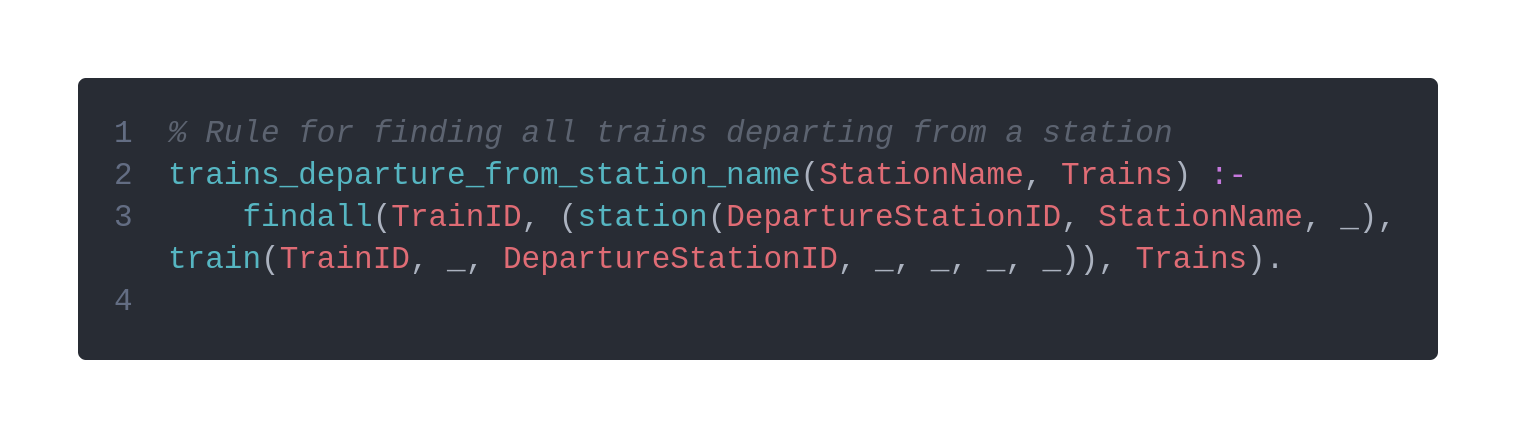
\includegraphics[width=370px]{img/code1}
				\caption{Regola n.1}
			\end{figure}
			
		\item Restituisce la lista di treni (\texttt{Trains}) che partono da una stazione specifica (\texttt{StationName}) a un determinato orario di partenza (\texttt{Departure});
			\begin{figure}[h]
				\centering
				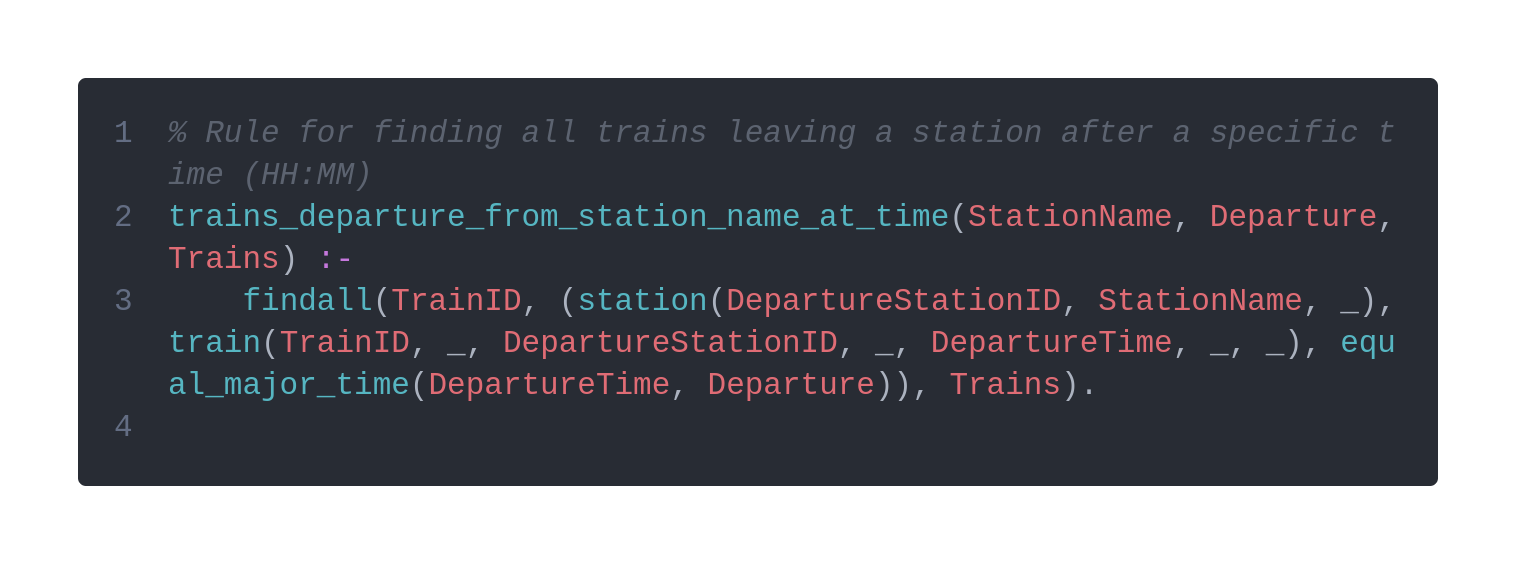
\includegraphics[width=370px]{img/code2}
				\caption{Regola n.2}

			\end{figure}
			\newpage
		\item Restituisce la lista di treni (\texttt{Trains}) che collegano due stazioni specifiche, partendo dalla stazione \texttt{DepartureStationName} e arrivando \texttt{ArrivalStationName} dopo un orario specifico \texttt{Time} (nella foramto HH:MM);
			\begin{figure}[h]
				\centering
				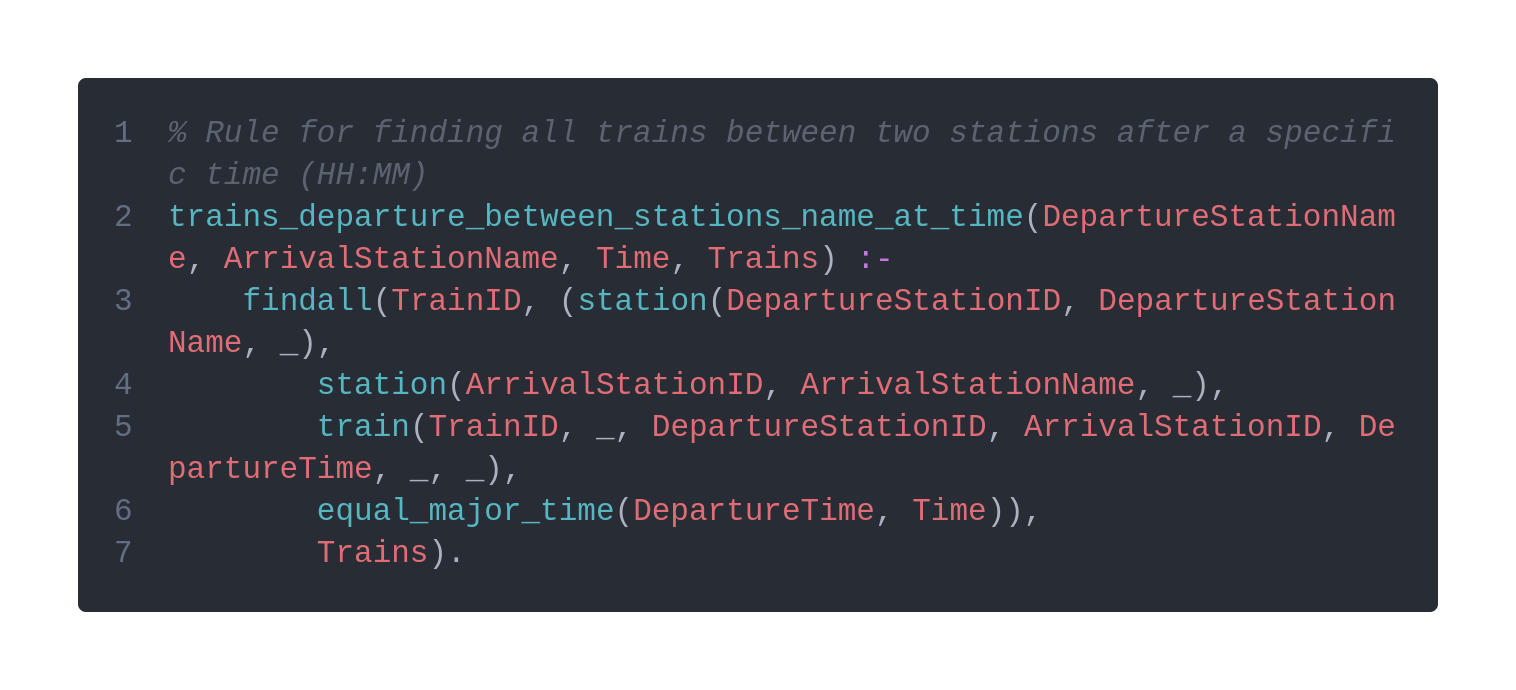
\includegraphics[width=370px]{img/code4}
				\caption{Regola n.3}

			\end{figure}
		\item Restituisce la lista di treni (Trains) che collegano due stazioni specifiche, partendo dalla stazione \texttt{DepartureStationName} e arrivando \texttt{ArrivalStationName};
			\begin{figure}[h]
				\centering
				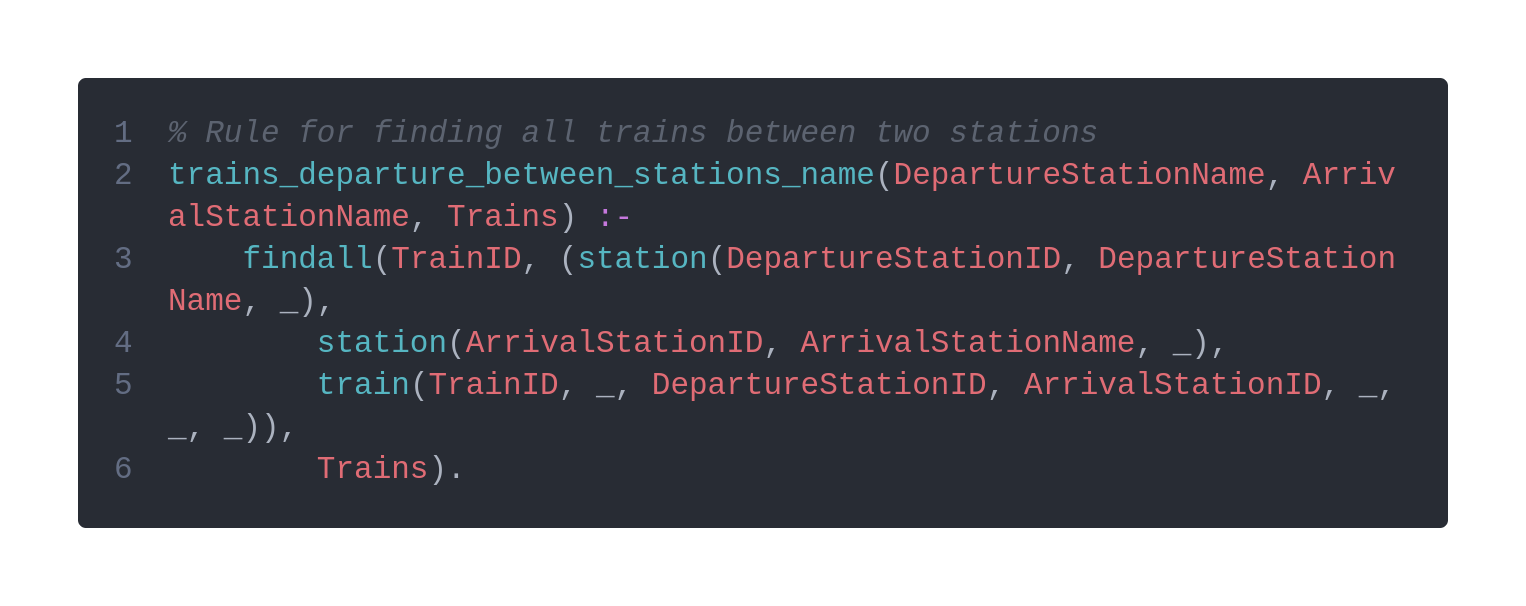
\includegraphics[width=370px]{img/code3}
				\caption{Regola n.4}

			\end{figure}

				
	\end{enumerate}
	
	
	Oltre queste query sono state prodotte altre regole, di supporto, per il funzionamento interno di queste principali, come quella per convertire le stringhe che rappresentano gli orari dal formato \texttt{"HH:MM"} in minuti, quella per reperire tutte le info dei treni dall'id, etc\dots

	\section{Machine Learning}
		Una delle funzionalità cardine del sistema è quella di predire se un treno sarà in ritardo, per implementrala è stato necessario addestrare un modello di Machine larning che in base a certe caratteristiche dello specifico treno farà una previsione più o meno corretta sul suo andamento. \\
		\linebreak
		In origine si è sperimentato con task di regressione, cioè, basandosi su un insieme di caratteristiche e dati, cercare di predire il valore esatto del ritardo, successivamente a causa di risultati non troppo ottmali ci si è spostati sul task di classificazione binaria, verrà predetto solo se un treno farà ritardo o meno.
	
	\subsection{Origine dataset}
		Il dataset di addestramento e test è stato recuperato per mezzo dell'interrogazione tramite API al serivio 	\href{http://www.viaggiatreno.it/infomobilita/index.jsp}{viaggiotreno.it}, in particolare si sono recuperate le informazoni giornaliere circa i treni (ID, tipo di treno, ...) ed in più il ritardo effettuato della corsa specifica fornendo così un insieme di dati essenziali per l'addestramento e la valutazione del modello di classificazione.
		
	\subsection{Analisi del dataset}
		Il dataset ottenuto è composto da circa 101169 osservazioni per otto features che, come già detto sopra, vanno a descrivere una serie di caratteristiche legate all'andamento giornaliero dei treni, abbiamo:
		
		\begin{enumerate}
			\item \textit{train\_id}[numeric]: identificatore univoco del treno;
			\item \textit{origin}[string]: nome della stazione di partenza;
			\item \textit{arrival}[string]: nome della stazione di arrivo;
			\item \textit{departure\_time}[string]: orario di partenza (HH:MM);
			\item \textit{arrival\_time}[string]: orario di arrivo (HH:MM);
			\item \textit{delay}[numeric]: ritardo registrato;
			\item \textit{train\_type}[string]: tipo di treno, regionale o nazionale;
			\item \textit{detection\_date}[date]: data della corsa.
		\end{enumerate}
		
			\begin{figure}[!h]
				\centering
				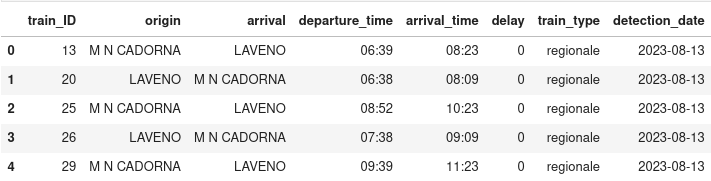
\includegraphics[width=1.1\linewidth]{img/dataset}
				\caption{Esempio delle prime istanze del dataset}
			\end{figure}
	

	\subsection{Preparazione dati}
		Prendendo il dataset così descritto ci sono una serie di problematiche da risolvere per poter usare i dati, in particolare andando a considerare le osservazioni notiamo che per i valori nominali, in questo caso quelli che esprimono il nome della stazione di partenza e di arrivo, ci sono dei caratteri che andrebbero modificati per formattare meglio il dataset, in particolare si sono andati a sostituire i punti, le virgole, gli accenti e le doppie virgolette con degli underscore per poter meglio gestire il dataset.
		
		\subsubsection{Analisi input features}
			Considerando le feature di input, cioè quelle sulle quali il modello andrà ad imparare, non tutte sono funzionali per per il raggiongimento del nostro scopo, in particolare si sono escluse:
			
			\begin{itemize}
				\item \textit{origin} (il modello scelto non accetta dati di tipo string);
				\item \textit{arrival} (il modello scelto non accetta dati di tipo string);
				\item \textit{detection\_date} (nessuna correlazione sulle feature su cui fare predizione).
			\end{itemize}
			Per quanto riguarda le feature rimanenti si è ritenuto opportuno includere nel learning anche \textit{train\_id} perchè si è osservato che determinati treni facevano sempre ritardo, inoltre si è optato per una trasformazionde dei valori per adattarli al modello, specificatamente i valori di \textit{departure\_time} e \textit{arrival\_time} da stringhe nel formato HH:MM si è passati a valori numerici che rappresentano i minuti ($hour*60+minutes$), inoltre si è operato anche su \textit{train\_type} eseguendo una binarizzazione:
			\begin{equation*}
				\begin{cases}
					1 \quad \text{if } train\_type(i) = regionale \\
					0 \quad \text{if } train\_type(i) = nazionale
				\end{cases}
			\end{equation*}
			
		\subsubsection{Analisi target feature}
			La target feature rappresenta l'biettivo sella notra predizione, in questo caso \textit{delay} che rappresenta il ritardo di una detrminata corsa, per la regressione lasciamo il valore così come ci viene dato, mentre per la classificazione anche in questo caso si è eseguita una binarizzazione:
			
			\begin{equation*}
				\begin{cases}
					1 \quad \text{if } delay(i) > 0  \\
					0 \quad \text{otherwise}
				\end{cases}
			\end{equation*}
			\linebreak
			\\
			Nel dataset abbiamo una distribuzione abbastanza bilanciata dei valori per la feature \textit{delay} ($41.3\%$ per treni in ritardo e $58.7\%$ per treni in orario), questo evita stategie per bilanciare i dati come data augmentation, cost-sensitive learning, etc\dots.
			
			\begin{figure}[!h]
				\centering
				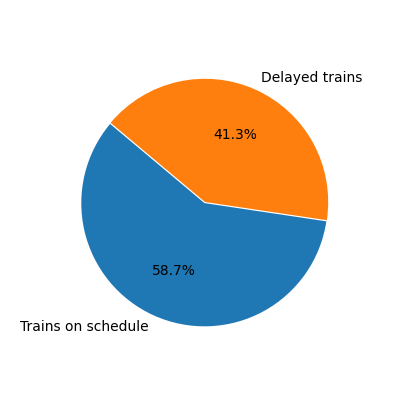
\includegraphics[width=270px]{img/delay_graph}
				\caption{Distribuzione dei treni con e senza ritardo}
			\end{figure}
			
	\subsection{Apprendimento automatico}
	Per produrre un sistema che va predire se un treno farà ritardo o meno si ricorre all'apprendimento automatico o \textit{machine learning} che consiste nell'addestrare un modello ad imparare dai dati e a migliorare le proprie prestazioni nei compiti specifici senza essere esplicitamente programmanti.\\
	Come già accennato si sono fatti esperimenti sia per la regressione che per la classificazione, in particolare per la prima si cerca di trovare una funzione $\hat{y}$, che meglio somiglia alla funzione "reale" che descrive i dati $y = f(X_1, X_2, \dots, X_n)$, mentre per la seconda si cerca di assegnare ad un'ovvervazione una certa categoria.

	\subsection{Random forest}
	Per questo caso speficico, sia per la regressione che per la classificazione si è usata la \textbf{Random forest}, modello di apprendimento automatico che combina molteplici alberi decisionali (\textit{decision trees}), entrando così nella categoria di modelli \textit{ensamble}, per migliorare la previsione e la generalizzazione.\\
	La random forest fa parte della gamma dei modelli di \textbf{apprendimento supervisionato}, cioè viene addestrato su un insieme di dati di addestramento che includono sia le caratteristiche (input features) che le risposte corrette (output features). 
	Il modello impara a fare previsioni basate su questi esempi etichettati.
		
	\begin{figure}[!h]
		\centering
		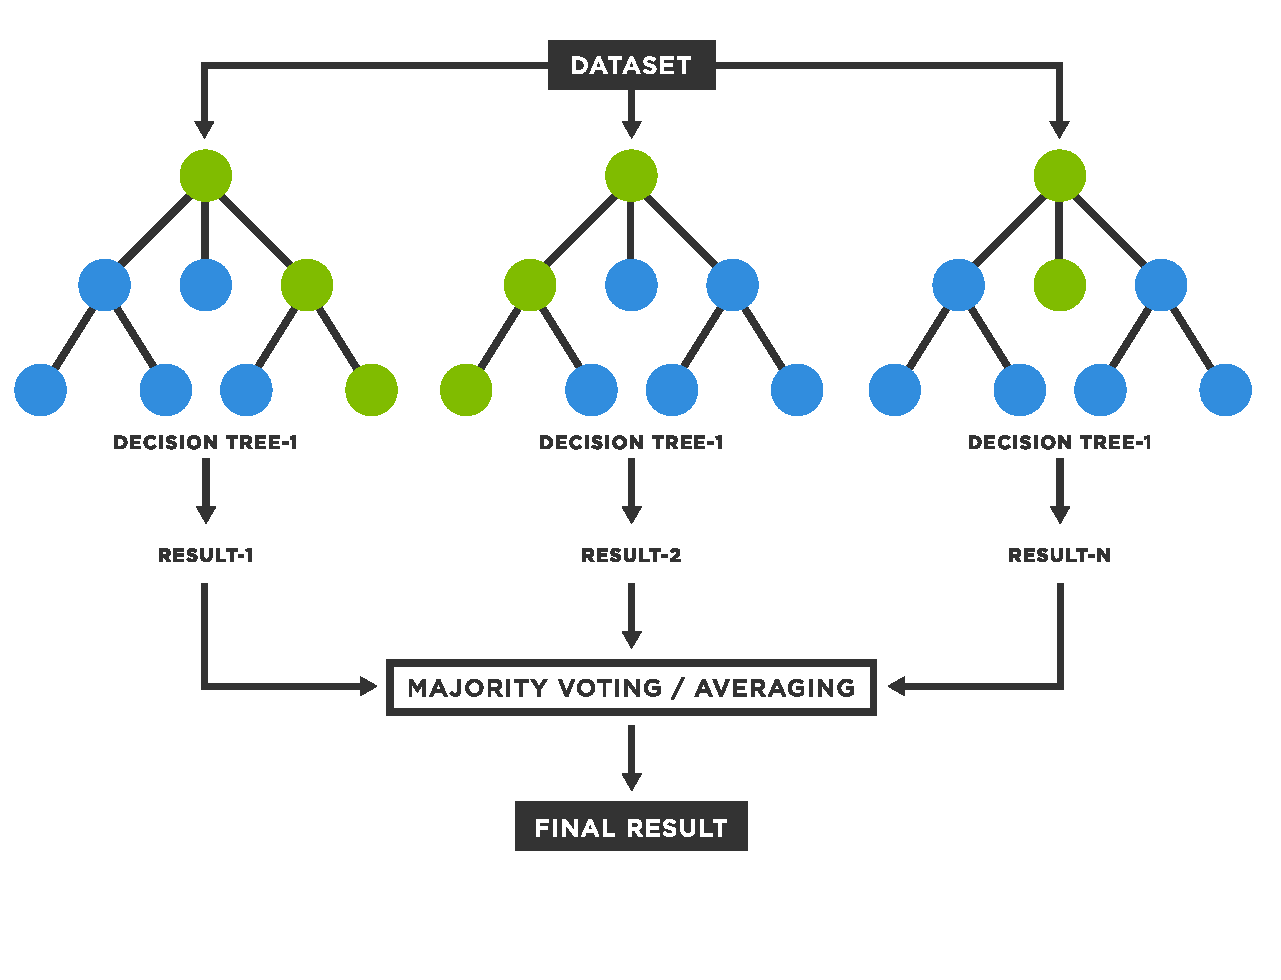
\includegraphics[width=270px]{img/random-forest-diagram}
		\caption{Esempio di random forest \href{https://www.spotfire.com/glossary/what-is-a-random-forest}{www.spotfire.com}}
	\end{figure}

	\subsubsection{Funzionamento}
	In particolare la Random Forest funziona creando un insieme di alberi decisionali (regressione/classificazione in base al task), ognuno addestrato su un subset casuale dei dati di addestramento e su un subset casuale delle caratteristiche.\\
	Questo processo introduce variabilità e riduce il rischio di sovradattamento (\textit{overfitting}) cioè quando il modello si lega troppo ai dati di \textit{training} risultando inefficacie su dati mai visti.\\ Quando si effettua una previsione, ciascun albero fornisce una previsione, e la Random Forest combina queste previsioni per ottenere un risultato finale più accurato e stabile.\\
	\linebreak
	Nel nostro caso per la regressione si è optato per una media delle predizioni di ogni albero, mentre per la classificazione la classe più predetta.
	\subsubsection{Configurazione scelta}
	Dopo varie sperimentazioni si riporta la migliore configurazione del modello, in particolare attraverso la libreria \texttt{scikit-learn} \cite{scikit_learn} si è definita una random forest le cui caratteristiche perculiari sono:\\
	\linebreak
	 \textbf{Regressione}
		\begin{enumerate}
			
			\item \texttt{n\_estimators = 35}, che rappresenta il numero di alberi su cui lavorare;
			\item  \texttt{criterion = "squared\_error"}, che rappresenta il criterio di \textit{split} degli alberi, in particolare il criterio è \textit{l'errore quadratico medio}, una misura che quantifica la differenza tra i valori previsti da un modello e i valori osservati o reali puntando a minimizzare la varianza, si calcola:
				$$MSE = \frac{1}{n}\sum_{i = 1}^{n}(y_i - \hat{y_i})^2$$
			dove:
				\begin{itemize}
					\item $n$ è il numero osservazioni;
					\item $y_i$ rappresenta il valore osservato (reale);
					\item $\hat{y_i}$ rappresenta il valore predetto.
				\end{itemize}

			Il criterio \texttt{squared\_error} è stato scelto per la sua efficacia e chiarezza di espressione, infatti è espresso nella stessa unità dei dati reali, in questo caso minuti di riatrdo, rendendo più comprensibile di quanto le previsioni del modello si discostano, in media, dai valori reali in termini di minuti.
			
		\end{enumerate}
		
		\textbf{Classificazione}
		\begin{enumerate}
			
			\item \texttt{n\_estimators = 50}, che rappresenta il numero di alberi su cui lavorare;
			\item  \texttt{criterion = "gini"},criterio di \textit{split} degli alberi, in particolare il criterio punta a minimizzare l'impurità dei nodi, quindi per scegliere l'attributo che meglio divide i dati in base alla target feature per ogni nodo si calcola:
			$$GINI(v) = 1-\sum_{i = 1}^{|c|}p_i^2$$
			dove:
			\begin{itemize}
				\item $v$ è il nodo in esame;
				\item $c$ rappresenta l'inseme delle classi;
				\item $p_i$ è la probabilità che un campione nel nodo $v$ appartenga alla classe $i$.
			\end{itemize}
			infine vene scelto il nodo con minor impurità. \\
			\linebreak
			L'indice \texttt{gini} è stato scelto per la sua efficenza, infatti la complessità per il calcolo dell'indice per uno nodo è dell'ordine di $O(c)$, dove c è il numero di classi.
			
		\end{enumerate}
	
	\subsection{Valutazione dei modelli}
	Per andare a valutare i modelli prodotti dopo l'addestramento si è usata la k-Fold-Cross-Validation, che esegue la riprtizione del dataset D in k sottoinsiemi (folds), $D_1, D_2, \dots , D_k$ prevede $k$ iterazioni ed all'$i$-esima iterazione il sottoinsieme $D_i$ sarà usato come dataset di test, metre l'unione degli altri sarà usata per allenare il modello. \\
	\linebreak
	Alla fine delle $k$ iterazioni, vengono raccolti i risultati delle valutazioni e calcolate le metriche di performance per valutare quanto bene il modello si comporta in media su dati di test diversi.
	
	\subsubsection{Metriche scelte regressione}
	Ai fini della valutazione si hanno a disposizione moltissime metriche adatte per moltissime situazioni, in questo caso speficiso si sono scelte:
	
	\begin{enumerate}
		\item Mean absolute error $(MEA)$ che misura la media degli errori assoluti tra le previsioni del modello e i valori osservati $$MAE = \frac{1}{n}\sum_{i = 1}^{n}|y_i - \hat{y_i}|$$
		\item Mean squared error $(MSE)$ che calcola la media dei quadrati degli errori tra le previsioni del modello e i valori osservati $$MSE = \frac{1}{n}\sum_{i = 1}^{n}(y_i - \hat{y_i})^2$$
		\item $R^2$-score, indica quanto il modello spiega le variazioni nei dati $$R^2 = 1 - \frac{\sum_{i=1}^{n}(y_i - \hat{y}_i)^2}{\sum_{i=1}^{n}(y_i - \bar{y})^2} $$
	\end{enumerate}
	
	dove:
	\begin{itemize}
		\item $n$ è il numero osservazioni;
		\item $y_i$ rappresenta il valore osservato (reale);
		\item $\hat{y_i}$ rappresenta il valore predetto;
		\item $\bar{y_i}$ rappresenta il valore medio.
	\end{itemize}

	
	\subsubsection{Metriche scelte classificazione}
	Per andare a valutare il modello prodotto si sono scelte le metriche più comuni:
	
	$$Precision = \frac{TP}{TP+FP} \quad Recall = \frac{TP}{TP+FN}$$

	Inoltre per avere un quadro della situazione più dettagliato si presentano altre mertiche che mettono in correlazione le due precedenti, come:
	
		
	\begin{enumerate}
		\item $f\beta-score$,  combinazione delle metriche classiche di $precision$ e $recall$ bilanciate da un parametro $\beta$ nella media armonica
		$$f\beta-score = \frac{(1+ \beta^2) \cdot Precision \cdot Recall}{\beta^2 \cdot Precision + Recall}$$
		\item $AUC-ROC$ (Area Under the Receiver Operating Characteristic Curve), area sotto la curva che rappresenta la relazione tra il tasso di veri positivi (True Positive Rate, TPR) e il tasso di falsi positivi (False Positive Rate, FPR) al variare della soglia di classificazione
		$$TPR = \frac{TP}{TP+FN} \quad FPR = \frac{FP}{FP+TN}$$
	
	\end{enumerate} 

	\subsection{Risultati}
		In questa sezione verranno riportati i risultati migliori di tutte le metriche discusse precedentemente:\\
		\linebreak
		\textbf{Regressione}:
		\begin{itemize}
			\item  \textbf{MAE}: 1.27;
			\item  \textbf{MSE}: 4.86;
			\item  \textbf{R$^2$ score}: 0.58;
		\end{itemize}
		
		\textbf{Classificazione}:
			\begin{itemize}
				\item \textbf{Precision}: 0.94;
				\item \textbf{Recall}: 0.86;
				\item \textbf{F2-score}: 0.92;
				\item \textbf{AUC-ROC}: 0.91.
				\item \textbf{Matrice di confusione}:
					\begin{center}
						\begin{blockarray}{*{2}{c} l}
							\begin{block}{*{2}{>{$\footnotesize}c<{$}} l}
								\texttt{Actual\_negative} & \texttt{Actual\_positive} & \\
							\end{block}
							\begin{block}{[*{2}{c}]>{$\footnotesize}l<{$}}
								11522 & 425 & \texttt{Predict\_negative} \\
								1107 & 7180& \texttt{Predict\_negative} \\
							\end{block}
						\end{blockarray}		
					\end{center}

					\begin{figure}[h]
					\centering
					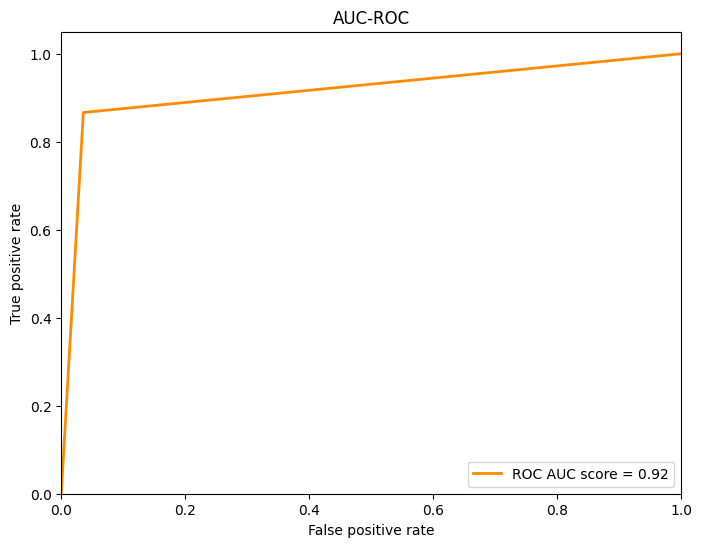
\includegraphics[width=245px]{img/roc_curve}
					\caption{Grafico AUC-ROC}
				\end{figure}
			\end{itemize}

			\subsection{Considerazioni}
				In generale il modello di classificazione mostra prestazioni solide, con un'accuratezza elevata, alta precisione e una buona capacità discriminativa. \\Tuttavia, il \textit{recall} è leggermente inferiore al 90\%, suggerendo possibili aree di miglioramento. L'\textit{F2-score} bilanciato fornisce un buon compromesso tra \textit{precision} e \textit{recall}, indicando un equilibrio nel modello. 

	\section{Interfaccia Grafica}
	Per interagire andare ad interagire con il sistema, all'avvio viene mostrato un menù, navigabile con i tasti direzionali "$\uparrow$" e "$\downarrow$", con tre opzioni:
	
		\begin{enumerate}
			\item \texttt{Cerca treno tra due stazioni}, per rintracciare tutti i treni tra la stazione di partenza e la stazione di arrivo dopo un determinato orario;
			\item \texttt{Cerca itinerario}, fornice un itinerario, cioè tutti le informazioni relative ai treni da prendere (orario, tipo, etc\dots) tra due stazioni;
			\item \texttt{Uscire}, per terminare l'applicazione.
		\end{enumerate} 
		Di seguito verranno riportate alcune immagini relative alla UI del sistema, includendo il menù principale e le diverse funzionalità:
		
		\begin{figure}[!h]
			\centering
			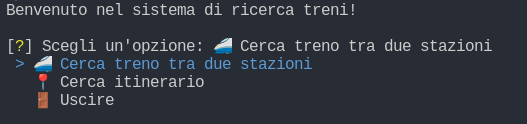
\includegraphics[width=400px]{img/main_menu}
			\caption{Distribuzione dei treni con e senza ritardo}
		\end{figure}

		\begin{figure}[!h]
			\centering
			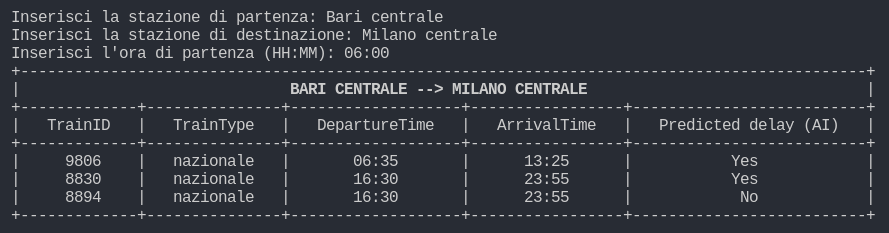
\includegraphics[width=400px]{img/search_train}
			\caption{Distribuzione dei treni con e senza ritardo}
		\end{figure}

		\begin{figure}[!h]
			\centering
			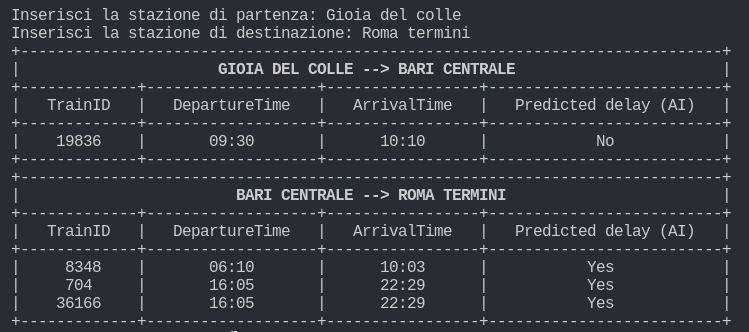
\includegraphics[width=400px]{img/search_itin}
			\caption{Distribuzione dei treni con e senza ritardo}
		\end{figure}
		
	\section{Conclusioni}
	
	L'obiettivo principale era sviluppare un sistema che potesse aiutare le persone a trovare la migliore soluzione per il viaggio in treno, andando a combinare la ricerca automatica di un itinerario che tenesse conto del numero di stazioni da percorrere e l'intelligenza artificiale per predire se il treno farà ritardo, andando così a limitare il disagio, in caso, da parte dei viaggiatori. \\
	\subsection{Rappresentazione e ricerca}
	Per la parte relativa alla ricerca, in primo luogo si sono reperiti i dati necessari attraverso chiamate API a vari servizi, successivamente si è andati a costruire una base di conoscenza (KB) per rappresentare formalmente la conoscenza ottenuta ed infine si è andati a progettare un grafo delle stazioni per applicare algoritmi di \textit{path-finding} in modo da minimizzare il numero di fermate.
	\subsection{Apprendimento}
	Per la seconda parte, relativa all'addestramento di un modello di machine learning con l'obiettivo di predire il ritardo di un treno, inizialmente si sono reperiti i dati relativi alle corse dei treni attraverso chiamate API giornaliere ai servizi precedentemente citati, successivamente si è analizzato il dataset formato, andando a eseguire una pre-eleborazione dei dati rimuovendo osservazioni problematiche per causa di dati mancanti, incoerenza e valori errati, eseguendo l'ingegnerizzazione delle feature separando le features di input da quelle di output, rimuovendone alcune e trasformandone i valori di altre.\\
	Come modello per addestrare si è selto la Random Forest, che combina vari alberi decisionali per fornire una previsione. \\
	I risultati ottenuti sono molto buoni avendo molti indicatori superiori al $90\%$, dimostrando la solidità del modello nel nostro contesto. \\
	\linebreak
	Consideando il tutto si piò dire di aver raggiunto l'obiettivo preposto, ottenendo un sistema efficente e soprattutto d'aiuto per noi viaggiatori.

	
	\section{Sviluppi futuri}
	Nonostante il buon funzionamento ed risultati ottenuti, il sistema presentato è aperto a sviluppi futuri che possano rendere il tutto ancora più efficiente e all'avanguardia. \\
	\linebreak
	Di seguito sono descritti alcuni dei possibili sviluppi futuri da esplorare:
	
	\begin{enumerate}
		\item Espansione della copertura ferroviaria andando a completare le informazioni relative a treni e staziono ed integrazione con altri servizi ferroviari come Italo, Frecciarossa, etc\dots;
		\item Miglioramento della ricerca andando a suggerire all'utente, sulla base dei caratteri inseriti, le stazioni che iniziano con quei caratteri;
		\item Integrazione di dati in tempo reale andando a fornire all'utente informazioni in \textit{real time};
		\item Creazione di client mobile per poter usare il sistema in mobilità.
	\end{enumerate}
	Queste sono alcune delle possibili migliorie/feature da poter implementare per rendere il sistema ancora più efficente e funzionale.
	\printbibliography
	
\end{document}